\documentclass[main.tex]{subfiles}

\begin{document}

\subsection{Secondo esercizio}
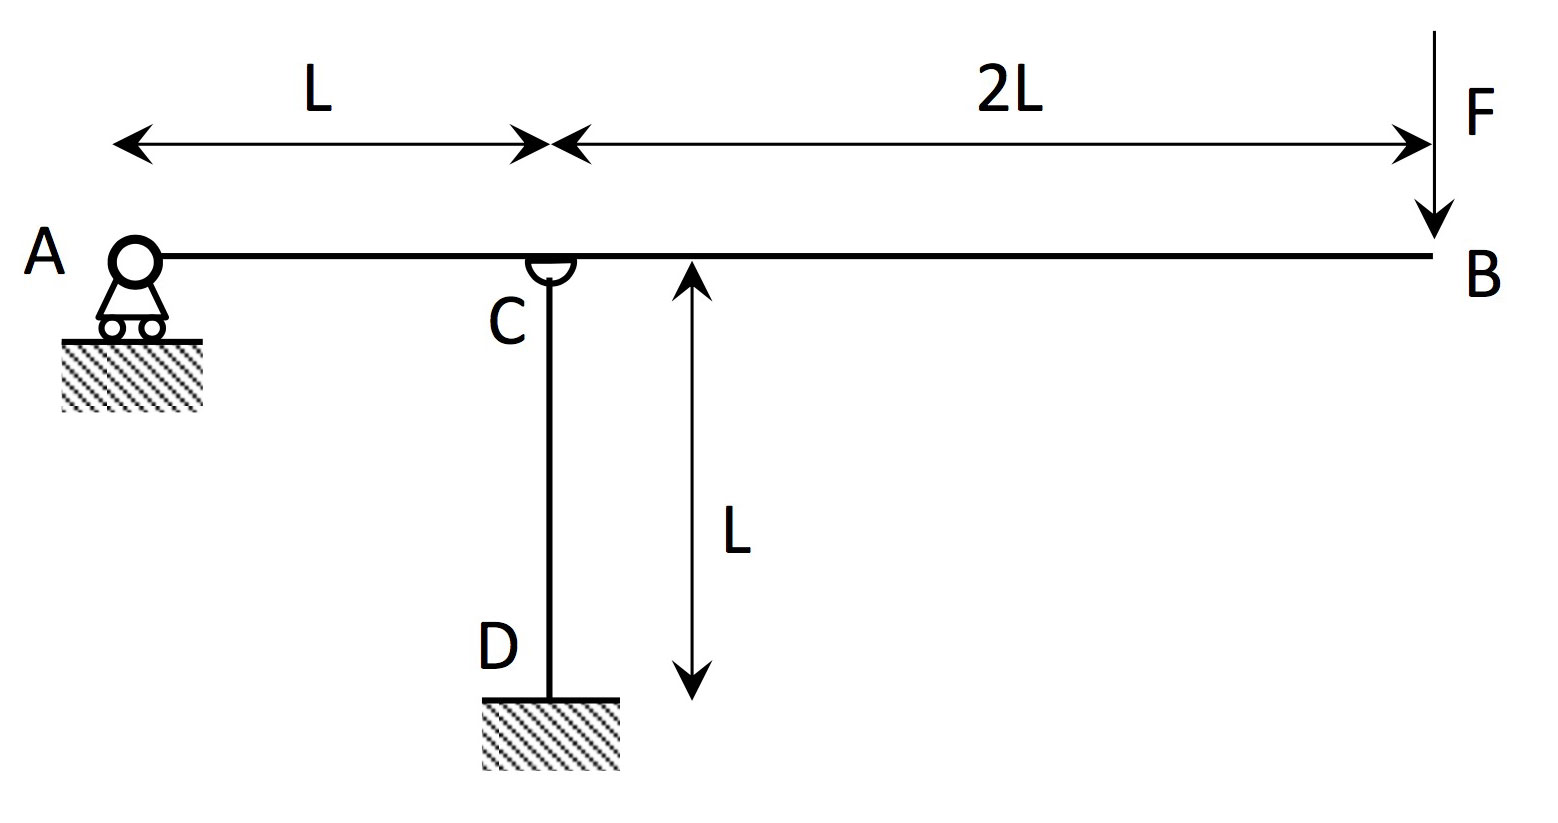
\includegraphics[width=\textwidth]{2015-0402-2.jpg}

La struttura in figura è soggetta alla sola forza verticale $F$.
Si chiede di calcolare:

\begin{enumerate}
\item Le reazioni vincolari a terra (punti A e D).
\item Le azioni interne nell’asta AB (disegnare i corrispondenti diagrammi).
\end{enumerate}
\clearpage

\subsection{Soluzione secondo esercizio (non verificata)}

\subsubsection{Osservazioni}

\begin{enumerate}
\item La struttura è formata da due aste, un vincolo a incastro, un vincolo a carrello ed una cerniera interna.
\end{enumerate}

\subsubsection{Analisi dei vincoli}
Tramite il computo dei gradi di vincolo possiamo fare una verifica preliminare si isostaticità:

\begin{figure}[H]
  \begin{subfigure}[b]{.5\textwidth}
  \centering
  \[
  	gdv: \begin{cases}
		gdv_{incastro} = 3\\
		gdv_{carrello} = 1\\
		gdv_{cerniera} = 2(2-1) = 2
  	\end{cases}
  \]
  \caption{Gradi di vincolo del sistema.}
  \end{subfigure}
  \hfill
  \begin{subfigure}[b]{.5\textwidth}
  \centering
  \[
  	gdl: \begin{cases}
  		gdl_{aste} = 6\\
  	\end{cases}
  \]
  \caption{Gradi di libertà del sistema.}
  \end{subfigure}
  \caption{Verifica preliminare di isostaticità.}
\end{figure}

Per la verifica preliminare, la struttura risulta isostatica.

\subsubsection{Primo punto}

\paragraph{Analisi dei vincoli esterni}
I vincoli ancorati a terra sono A e D:

\begin{figure}[H]
\centering
\resizebox{.5\textwidth}{!}{% First image 2015 06 29

\begin{tikzpicture}

  \tiny


  \point{c}{0}{0}
  \point{c1}{0}{0.8}
  \point{c2}{-0.8}{0}
  \point{a}{2-1.41421}{1.41421}
  \point{a1}{2-1.41421}{0.8+1.41421}
  \point{d}{2}{0}
  \point{b}{2+1.41421}{-1.41421}
  \point{b1}{2+1.41421}{-1.41421-1.3}

  \beam{2}{c}{d}[0][1];
  \beam{2}{a}{b};

  \load{1}{a}[180][0.5]
  \load{1}{a1}[270][0.5]

  \load{2}{c}
  \load{1}{c}[180][0.5]
  \load{1}{c}[270][0.5]

  \load{1}{b1}[90][1]

  \notation{1}{c}{$\vec{M}_C$}[below right]
  \notation{1}{c}{$\vec{H}_C$}[below left]
  \notation{1}{c}{$\vec{V}_C$}[above right]

  \notation{1}{a}{$\vec{H}_A$}[below left]
  \notation{1}{a}{$\vec{V}_A$}[above right]

  \notation{1}{b}{$\vec{F}$}[below right]

  % \notation{1}{a1}{$\vec{H}_A$}
  % % \notation{1}{d1}{$\vec{R}_D$}
  % % \notation{1}{b1}{$\vec{H}_B$}[below left]
  % \notation{1}{c1}{$\vec{F}$}[above left]

  %  % \support{3}{o};

  %  % %Degrees
  %  % \notation{1}{o}{$\alpha$}[above];
  %  % \notation{1}{a}{$\beta$}[above];

  %  % \notation{5}{o}{a}[$a$];
  %  % \notation{5}{a}{b}[$b$];
  %  % \notation{5}{o}{b}[$c$];

\end{tikzpicture}}
\caption{Reazioni vincolari dei vincoli esterni}
\end{figure}

\[
\begin{cases}
	V_A + V_D= F \\
	H_D = 0 \\
	M_D + LV_A + 2LF = 0
\end{cases}
\]

\paragraph{Analisi delle reazioni vincolari nell'asta CD}

\begin{figure}[H]
\centering
\resizebox{.25\textwidth}{!}{% First image 2015 06 29

\begin{tikzpicture}

  \tiny


  \point{a}{0}{0}
  \point{c}{1}{0}
  \point{b}{3}{0}
  \point{d}{1}{-1}


  \beam{2}{d}{c};

  \load{1}{d}[270][0.5]
  \load{2}{d}

  \load{1}{c}[0][0.5]
  \load{1}{c}[90][0.5]


  \notation{1}{d}{$\vec{M}_D$}[above]
  \notation{1}{d}{$\vec{H}_D$}[below left]
  \notation{1}{d}{$\vec{V}_D$}[below right]

  \notation{1}{c}{$\vec{V}_C$}[above right]
  \notation{1}{c}{$\vec{H}_C$}[below right]

\end{tikzpicture}}
\caption{Reazioni vincolari nell'asta AB}
\end{figure}

\[
\begin{cases}
	V_C = V_D\\
	H_C = 0\\
	M_D = 0
\end{cases}
\]

Sostituisco le identità ottenute nel sistema precedente ed ottengo:

\[
\begin{cases}
	V_D= 3F \\
	H_D = 0 \\
	V_A = -2F
\end{cases}
\]

\subsubsection{Secondo punto}
I tre vettori possiedono unicamente componenti di taglio.

\paragraph{Sforzo normale}

\begin{figure}[H]
\centering
\resizebox{.3\textwidth}{!}{% First image 2015 06 29

\begin{tikzpicture}

  \tiny


  \point{c}{0}{0}
  \point{a}{0}{1}
  \point{b}{1}{0}
  \point{d}{2}{0}

   \beam{2}{c}{d}[0][1];

  \internalforces{c}{b}{1}{1}[0][blue];

\end{tikzpicture}}
\caption{Grafico sforzo normale nell'asta AB}
\end{figure}

\paragraph{Taglio}
In questo caso, il taglio coincide con il valore dei vettori che agiscono sull'asta.

Partendo da sinistra, il vettore $V_A$ impone una rotazione \textbf{anti-oraria} al tronco AC, mentre il vettore $V_D$ va ad imporre una rotazione oraria con $F$ nel tronco di destra CB.

\begin{figure}[H]
\centering
\resizebox{.3\textwidth}{!}{% First image 2015 06 29

\begin{tikzpicture}

  \tiny


  \point{c}{0}{0}
  \point{c1}{0}{0.8}
  \point{c2}{-0.8}{0}
  \point{a}{2-1.41421}{1.41421}
  \point{a1}{2-1.41421}{0.8+1.41421}
  \point{d}{2}{0}
  \point{d1}{2-0.8}{0}
  \point{b}{2+1.41421}{-1.41421}
  \point{b1}{2+1.41421}{-1.41421-1.3}

  \beam{2}{a}{b};

  \internalforces{a}{d}{-0.707}{-0.707}[0][blue];
  \internalforces{d}{b}{0.707}{0.707}[0][red];

\end{tikzpicture}}
\caption{Grafico taglio nell'asta AB}
\end{figure}

\paragraph{Momento flettente}

\[
	M_{max} = 2LF
\]

Il momento aumenta linearmente fino a raggiungere il massimo nel punto C, in cui la forza $V_D$ viene applicata, che impone un momento negativo e porta a decrescere linearmente il momento flettente sino a raggiungere 0 nell'estremo opposto.
\\
Le fibre tese risultano sul lato superiore.

\begin{figure}[H]
\centering
\resizebox{.3\textwidth}{!}{% First image 2015 06 29

\begin{tikzpicture}

  \tiny


  \point{c}{0}{0}
  \point{c1}{0}{0.8}
  \point{c2}{-0.8}{0}
  \point{a}{2-1.41421}{1.41421}
  \point{a1}{2-1.41421}{0.8+1.41421}
  \point{d}{2}{0}
  \point{d1}{2-0.8}{0}
  \point{b}{2+1.41421}{-1.41421}
  \point{b1}{2+1.41421}{-1.41421-1.3}

  \beam{2}{a}{b};

  \internalforces{a}{d}{0}{-0.707}[0][red];
  \internalforces{d}{b}{-0.707}{0}[0][red];

\end{tikzpicture}}
\caption{Grafico momento flettente nell'asta AB}
\end{figure}

\end{document}